\documentclass[12pt]{article}
\usepackage{graphicx}
\usepackage{pdfpages}

\begin{document}
\noindent
Andrew Brandt
9-17-22

\vspace{5mm}

\Large\noindent
The first thing that comes to mind is to solve the inputs for a value.
There were three possible answers given for number one. Two of them did not work because there are only certain numbers that can be used.

\[(2*4)-(1-7)\]

\[5+2*1-6\]

\[(3*4)/6-1\]

\vspace{5mm}

\noindent Evaluating each of these equals 1.

\vspace{5mm}

\noindent Before I go any further, I need to look at the assumptions that I have just made.

\begin{enumerate}
    \item The order of operations that is being used
    \item the arrangement of the numbers
\end{enumerate}

\vspace{5mm}

\noindent I am assuming the standard order of operations described in the PEMDAS acronym. Based on the inputs that did not work due to the limited numbers that can be used,
I have come to assume that the arrangement of the numbers does not matter as long as it equals the correct number.

\noindent If I assume that the key to open the door is making the numbers equal the door number, then the second door must equal 2

\[(3*4)/(6*1)\]

\vspace{5mm}
\noindent Once again, using the assumed order of operations, the numbers equal 2, corresponding to the door number
\vspace{5mm}
\noindent With the given information, we can check this one more time for the third door.
\vspace{5mm}
\[1+(3*4)/6\]
\vspace{5mm}
\noindent This does in fact once again correspond to the door number.
\vspace{5mm}
\noindent Now I want to review my rules for opening the door before I try to unlock the rest of the doors
\vspace{5mm}
\begin{enumerate}
    \item Only the numbers 1,3,4 and 6 can be used
    \item An operator must separate all the digits
    \item No fractions
    \item only +,*,/,- can be used
    \item all of the four possible digits must be used
\end{enumerate}
\vspace{5mm}
\noindent This seems good enough, but can these four digits really be arranged to equal numbers 1-32?
\vspace{5mm}
\includepdf[pages={2}]{sol.pdf}
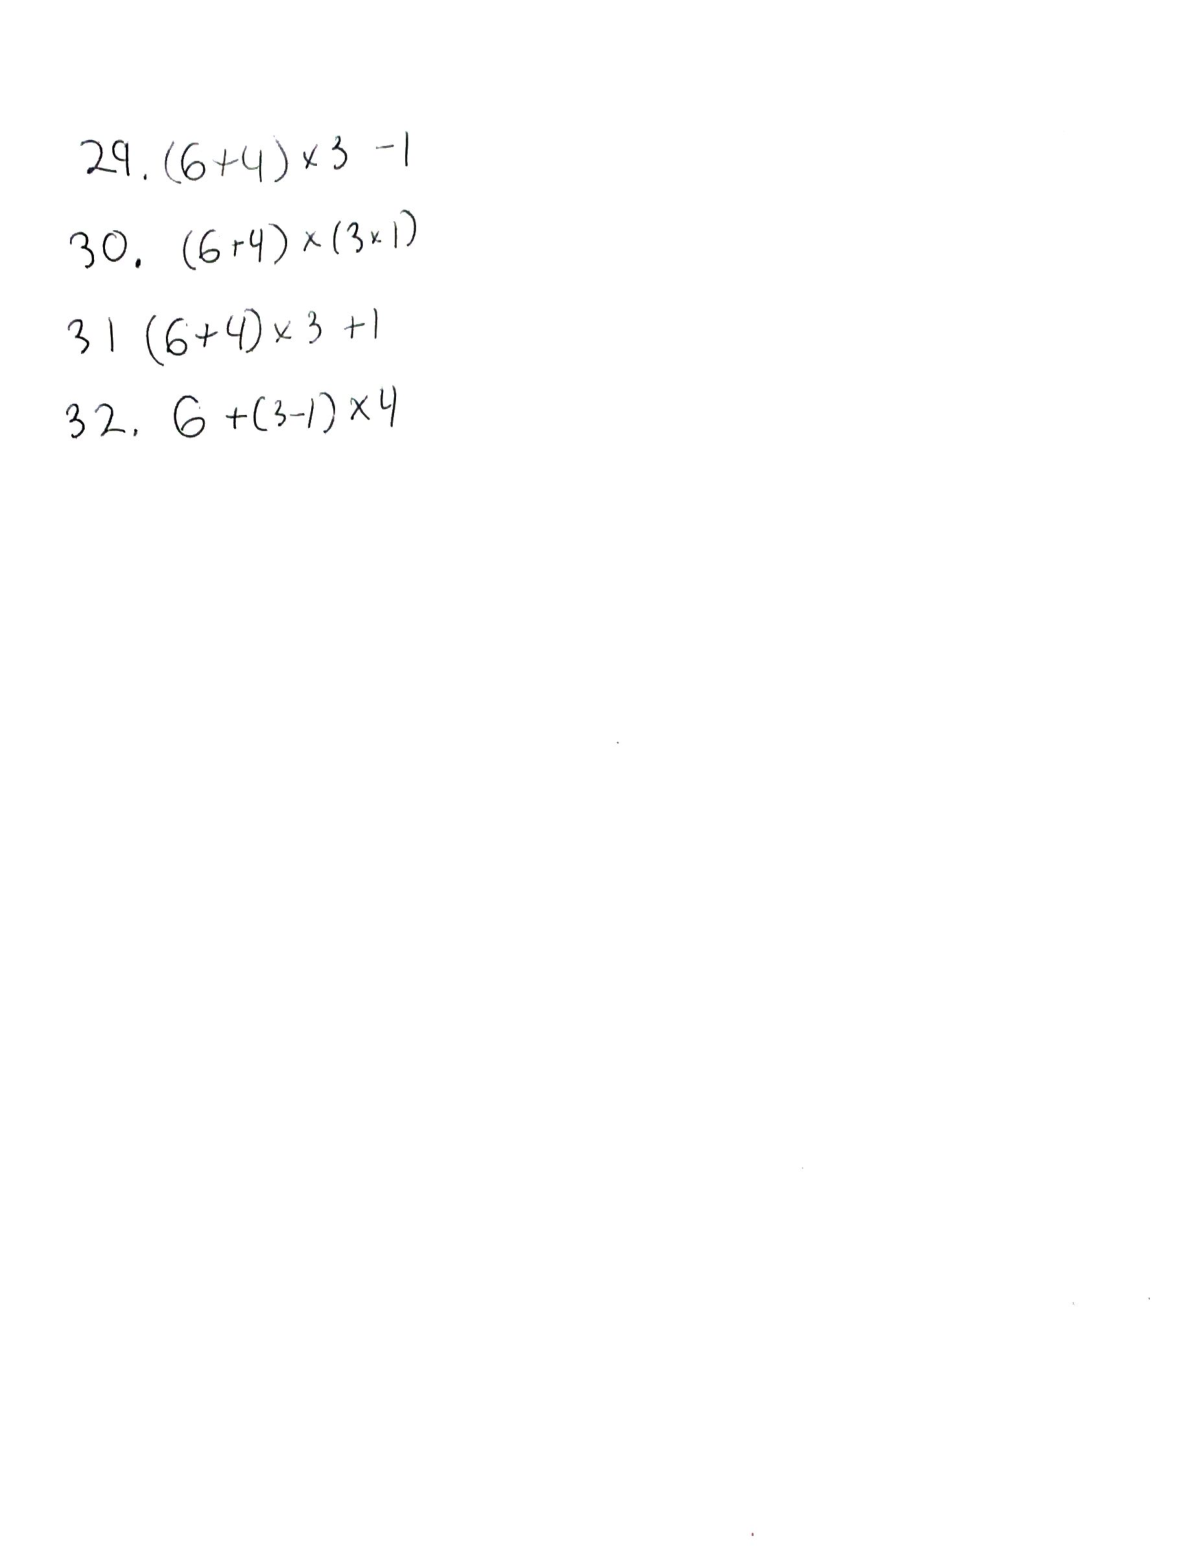
\includepdf[pages={1}]{sol.pdf}

\vspace{5mm}
\noindent The general solution for these doors was mostly brute force.
However, once a brute force solution is found, rearranging the numbers can yield many more solutions.
Through this method, many solutions can be found in a short amount of time, but they will not be in order.

\vspace{5mm}
\noindent 
The brute force of the solution includes 4 possible numbers and 4 possible expressions.
All four numbers must be used, but only 3 operators are used per solution. so it would be 4 factorial and 3 to the 4.
I think this would yield a n to the n solution.

\end{document}
